\documentclass[11pt]{article}
\usepackage[margin=1in]{geometry}
\usepackage{booktabs}
\usepackage{graphicx}
\usepackage{hyperref}
\usepackage{amsmath,amssymb}
\usepackage{subcaption}
\usepackage{titlesec}
\titleformat*{\section}{\large\bfseries}
\titleformat*{\subsection}{\normalsize\bfseries}

\title{What Do Citation-Based Classifiers Actually Measure?\\
       \large A Multi-Probe Study of Impact vs.\ Novelty in HCI Papers}
\author{Xiaohan Ye \\ STATS 507 --- Final Project}
\date{April 21, 2026}

\begin{document}
\maketitle

\begin{abstract}
Citation-based classifiers are commonly proposed as proxies for identifying important or novel research. We train standard TF-IDF and Sentence-BERT classifiers on a 2{,}365-paper Human--Computer Interaction (HCI) corpus drawn from OpenAlex (2010--2023), labelling papers as ``high-impact'' by within-year citation percentile. We then probe what the classifiers actually capture along three independent axes: (i) lexical novelty (first-year-of-appearance of $n$-grams), (ii) semantic novelty (cosine distance to the prior-year embedding centroid), and (iii) temporal generalisation (train-cutoff $\to$ future-year decay). We find that the impact classifiers correlate weakly with one novelty probe and modestly with the other (Spearman $\rho \in [-0.01,\, +0.27]$, all 95\% bootstrap CIs near zero), the two novelty probes themselves disagree ($\rho \approx -0.05$), and PR-AUC drops $\sim$10\% as the train$\to$test gap grows from one to three years. Inspection of the TF-IDF model's coefficients confirms it learns popular subfield vocabulary and writing-style cues---not novelty. We argue this is a critical caveat for anyone deploying citation-trained classifiers as research-trend or novelty detectors, and that ``novelty'' itself is not a single quantity.
\end{abstract}

\section{Introduction}
The original goal of this project was to build a temporal NLP pipeline to detect ``concept-introducing'' papers. We quickly discovered that no widely-available labelled corpus of ``novel concept'' introductions exists, and that weakly-supervised novelty heuristics are noisy. After consultation with course staff, we considered the common workaround of using citation counts as a proxy. This pivots the question from \emph{what makes a paper novel?} to a more answerable empirical one: \textbf{if we train a standard text classifier to predict highly-cited papers, what does the model actually learn---and is it a defensible proxy for novelty?}

This report's contribution is the probe answering that question, hardened with bootstrap confidence intervals, permutation tests, two independent novelty signals, and a temporal-drift experiment. Our finding is negative-but-useful: impact classifiers are largely orthogonal to corpus-novelty signals; novelty is itself multi-dimensional; and the classifier's predictive power decays over time.

\section{Data}
We pulled 22{,}297 HCI-related papers from OpenAlex via the \texttt{pyalex} client, restricting to the HCI concept (\texttt{C107457646}) and years 2010--2023, capping at 1{,}600 papers/year ranked by citation count. We then filtered to papers whose \textbf{top-5 OpenAlex concepts} explicitly include ``Human--computer interaction'' (note: en-dash U+2013, not a hyphen---a real source of bugs in OpenAlex tooling), yielding 3{,}935 papers. Survey/review/meta-analysis papers were excluded by regex on the title and abstract prefix; surveys are a known citation-count artifact that would otherwise dominate the positive class.

\paragraph{Labelling.} For each paper, we computed its citation-count percentile \emph{within its publication year} to remove age bias. Top-10\% papers are positive, bottom-50\% are negative, the middle 40\% is discarded. The labelled set contains 2{,}365 papers (399 positive, 1{,}966 negative; positive rate $\approx 16.9\%$ in every split).

\paragraph{Splits.} Strictly time-based: train $\le 2019$ ($n=1{,}833$), val 2020--2021 ($n=262$), test 2022--2023 ($n=270$). No paper appears in more than one split.

\begin{figure}[h]\centering
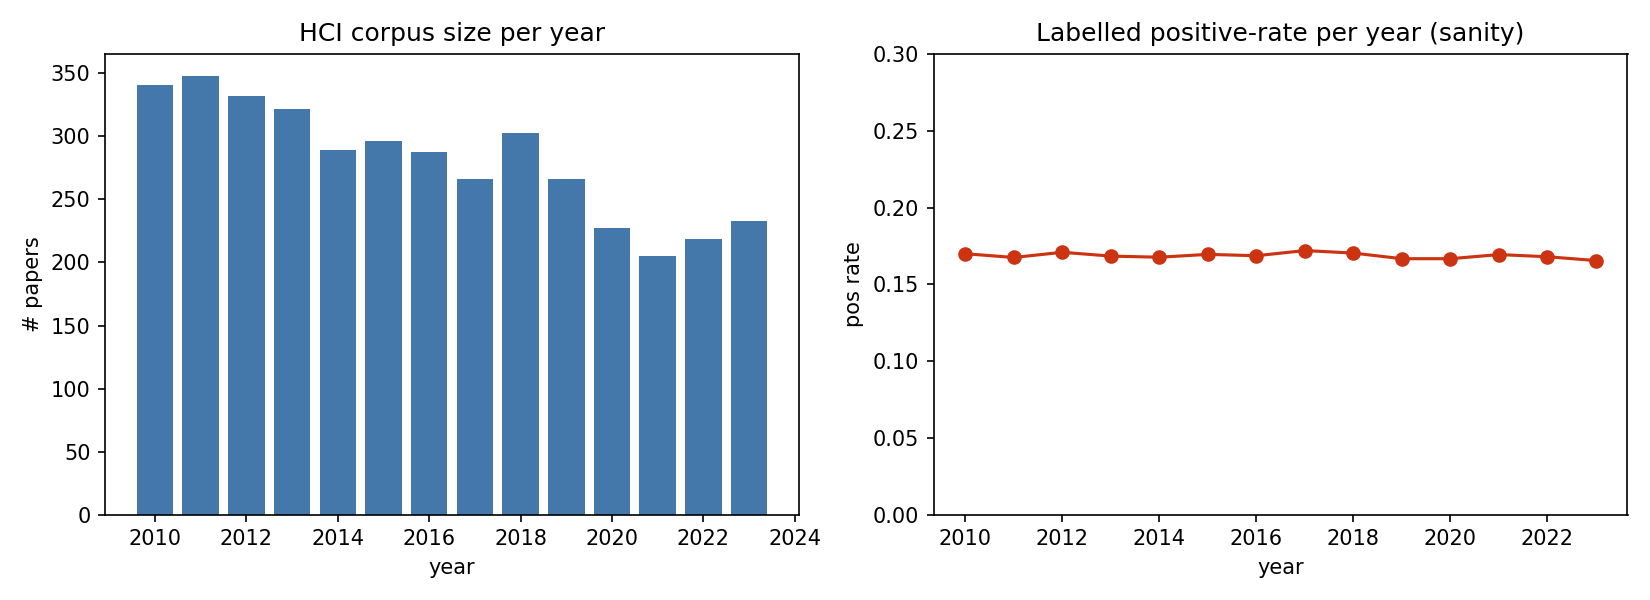
\includegraphics[width=0.95\linewidth]{figures/per_year_stats.png}
\caption{Left: HCI-filtered corpus size per year. Right: positive-rate in the labelled set per year is approximately constant ($\approx 0.17$), confirming that within-year percentile labelling removes age bias.}
\label{fig:per_year}
\end{figure}

\section{Methods}
\subsection{Impact classifiers}
Two models, both trained on \texttt{title + " " + abstract}:
\begin{itemize}
  \item \textbf{TF-IDF + LR}: \texttt{TfidfVectorizer(ngram\_range=(1,2), min\_df=5, max\_features=50k, sublinear\_tf=True)} $\to$ \texttt{LogisticRegression(class\_weight='balanced', C=1, max\_iter=1000)}.
  \item \textbf{Sentence-BERT (all-MiniLM-L6-v2) + LR}: 384-dim embeddings, \texttt{StandardScaler}, then the same logistic regression.
\end{itemize}
Decision thresholds are tuned on the validation set ($F_1$-maximising sweep over $[0.10, 0.90]$ in 0.05 steps), then frozen for test evaluation.

\subsection{Two independent novelty probes}
\textbf{Lexical (n-gram) novelty.} For each paper we extract unigram, bigram, and trigram phrases (lowercased, stop-listed). Across the full HCI corpus we record the \emph{first year} each phrase appears. The \textbf{n-gram novelty score} is the fraction of a paper's phrases (corpus frequency $\ge 2$) whose first appearance is the paper's own publication year.

\textbf{Semantic novelty.} Using MiniLM embeddings of \texttt{title + abstract}, we compute the centroid of all prior-year embeddings, and define a paper's \textbf{semantic novelty} as $1 - \cos(\text{paper}, \text{prior-centroid})$. A paper far from the prior-year cloud is semantically novel.

Both probes use only text, year, and the corpus---no labels, no citations, no classifier predictions. Any correlation between either probe and the impact classifier is therefore genuine information about what the classifier captures. The two probes capture different intuitions (\emph{new words} vs.\ \emph{new geometry}), and we will show they only weakly agree---an important nuance.

\subsection{Robustness apparatus}
For every reported metric and correlation we provide 95\% bootstrap confidence intervals ($B=2000$ resamples). For Spearman correlations between classifier scores and novelty probes we additionally report a permutation $p$-value ($B=2000$ shuffles of the novelty vector). For temporal drift we sweep training cutoffs $Y \in \{2014, \ldots, 2020\}$ and evaluate at gaps $\{1,2,3\}$ years forward.

\section{Results}
\subsection{Baselines and model performance (test set)}
\begin{table}[h]\centering
\begin{tabular}{lrrrrrr}
\toprule
model & $n$ & precision & recall & $F_1$ & ROC-AUC & PR-AUC \\
\midrule
majority class & 270 & 0.000 & 0.000 & 0.000 & 0.500 & 0.167 \\
random (prior) & 270 & 0.146 & 0.133 & 0.139 & 0.498 & 0.153 \\
\textbf{TF-IDF + LR} & 270 & 0.148 & 0.200 & 0.170 & 0.570 & 0.181 \\
\textbf{Embed + LR}  & 270 & 0.138 & 0.467 & 0.213 & 0.471 & 0.172 \\
\bottomrule
\end{tabular}
\end{table}

With bootstrap CIs (95\%): TF-IDF $F_1 = 0.170~[0.076, 0.273]$, PR-AUC $= 0.181~[0.134, 0.253]$; Embed $F_1 = 0.213~[0.140, 0.292]$, PR-AUC $= 0.172~[0.119, 0.266]$. The two models are statistically indistinguishable on PR-AUC; both clear the random PR-AUC of 0.153 only by a thin margin.

\begin{figure}[h]\centering
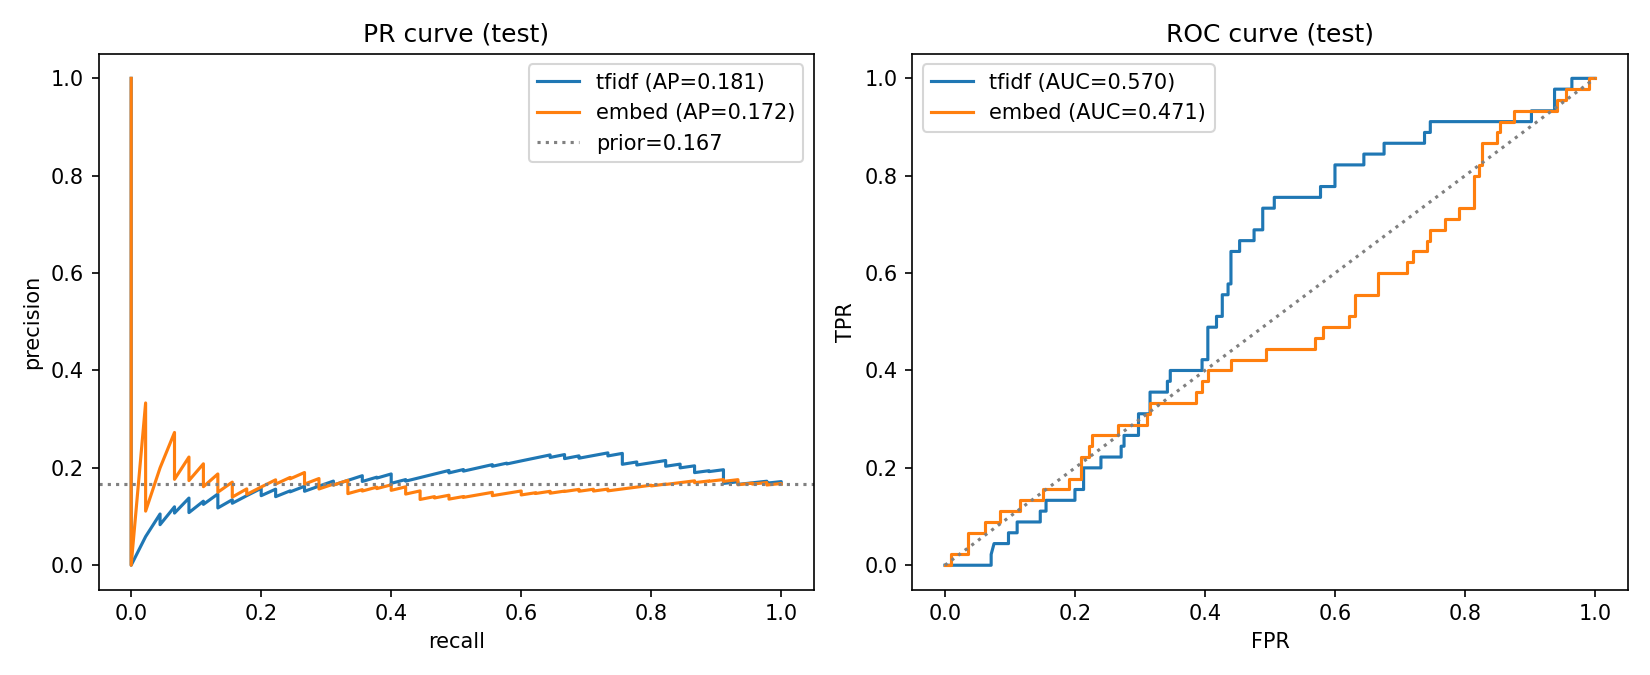
\includegraphics[width=0.95\linewidth]{figures/pr_roc.png}
\caption{Precision-recall (left) and ROC (right) curves for both classifiers on the test set. The TF-IDF model dominates in the high-precision regime; the embedding model is more uniform but its ROC dips below the diagonal at high FPR, reflecting noise on a small test set.}
\label{fig:prroc}
\end{figure}

\begin{figure}[h]\centering
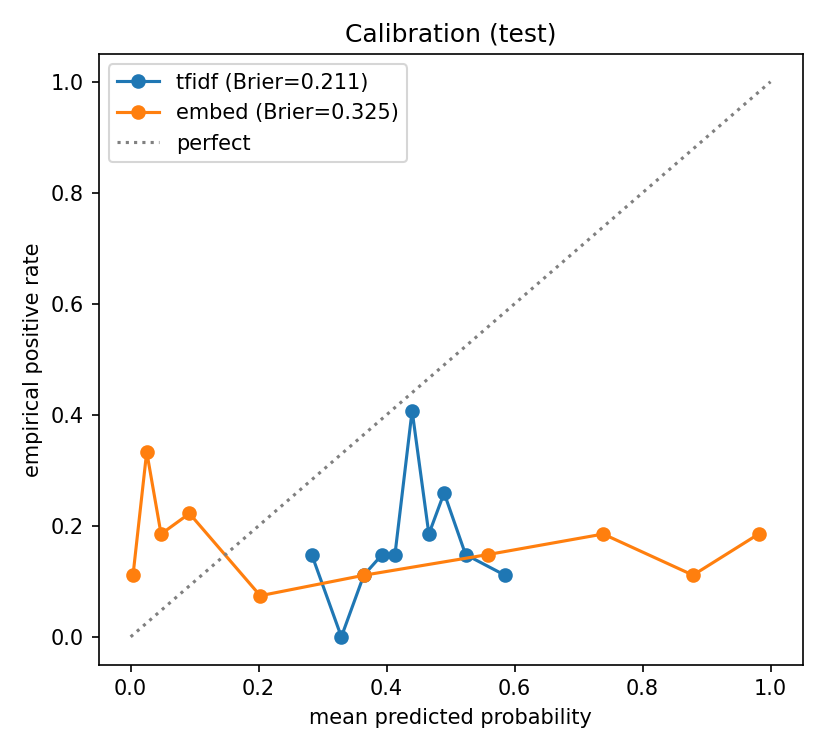
\includegraphics[width=0.6\linewidth]{figures/calibration.png}
\caption{Reliability diagrams (10 quantile bins). Both classifiers are systematically over-confident in the high-probability bin, a known consequence of \texttt{class\_weight=balanced} on imbalanced data. Brier scores are reported in the legend.}
\label{fig:calib}
\end{figure}

\subsection{Impact vs.\ novelty: bootstrap CIs and permutation tests}

\begin{table}[h]\centering
\begin{tabular}{llrrrr}
\toprule
model & probe & Spearman $\rho$ & 95\% CI & perm.\ $p$ \\
\midrule
TF-IDF & n-gram     & $+0.130$ & $[+0.014,\, +0.251]$ & $0.035$ \\
TF-IDF & semantic   & $+0.269$ & $[+0.163,\, +0.374]$ & $<0.001$ \\
Embed  & n-gram     & $-0.013$ & $[-0.133,\, +0.105]$ & $0.815$ \\
Embed  & semantic   & $+0.101$ & $[-0.016,\, +0.231]$ & $0.096$ \\
\bottomrule
\end{tabular}
\end{table}

Three of the four correlations are statistically near zero; only TF-IDF--vs--semantic-novelty rises to $\rho = 0.27$, which is a real but modest signal. Even the largest effect leaves more than 92\% of variance unexplained. \textbf{Highly cited and highly novel are not the same axis.}

\begin{figure}[h]\centering
\begin{subfigure}{0.48\linewidth}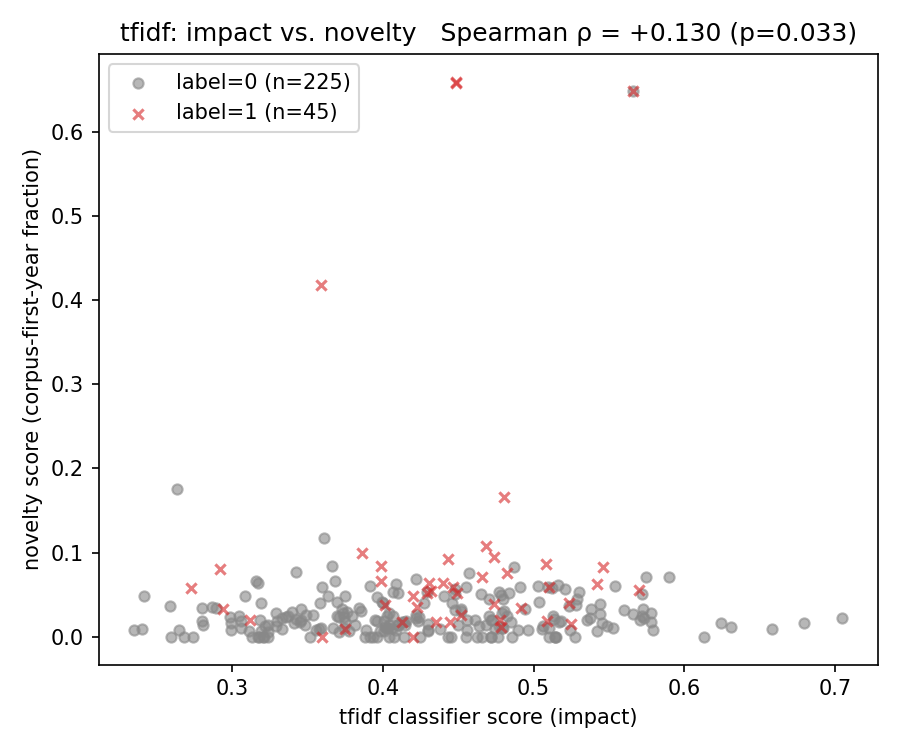
\includegraphics[width=\linewidth]{figures/scatter_tfidf.png}\caption{TF-IDF vs.\ n-gram novelty}\end{subfigure}
\begin{subfigure}{0.48\linewidth}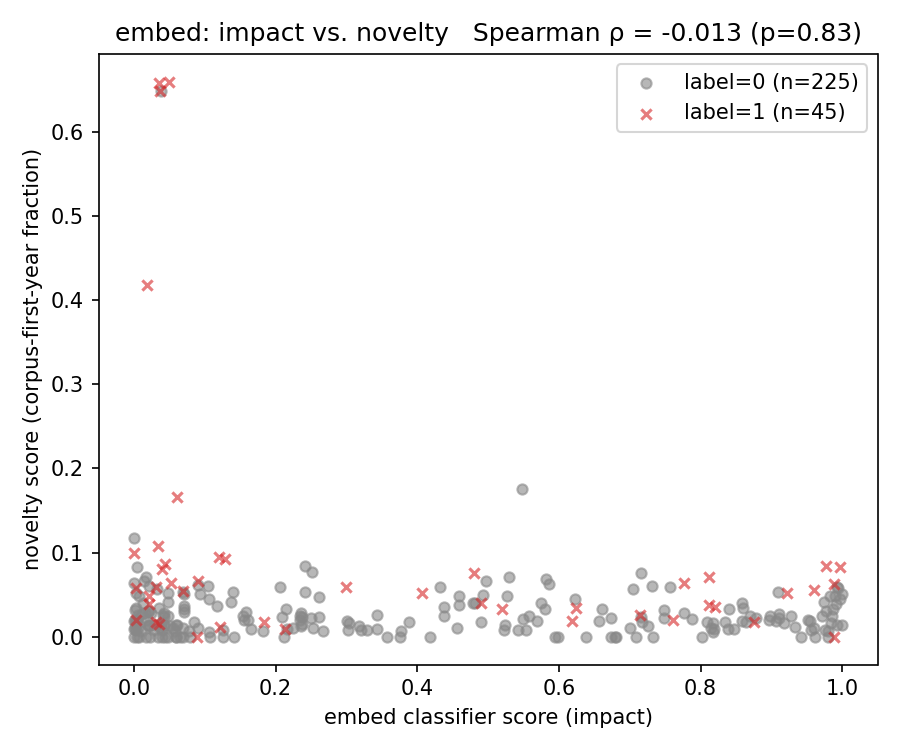
\includegraphics[width=\linewidth]{figures/scatter_embed.png}\caption{Embed vs.\ n-gram novelty}\end{subfigure}
\caption{Joint distributions of impact-score and n-gram novelty-score on the test set.}
\label{fig:scatter}
\end{figure}

\subsection{The two novelty probes disagree}
A subtle and important secondary finding: the two novelty probes themselves are essentially uncorrelated (Spearman $\rho = -0.047$ across the labelled set; Figure~\ref{fig:probes}). \textbf{``Novelty'' is not a single quantity}: lexical novelty (a paper introducing new vocabulary) and semantic novelty (a paper sitting far from the prior-year cloud) measure genuinely different things. This is why our impact classifier's relationship to ``novelty'' depends on which probe you use.

\begin{figure}[h]\centering
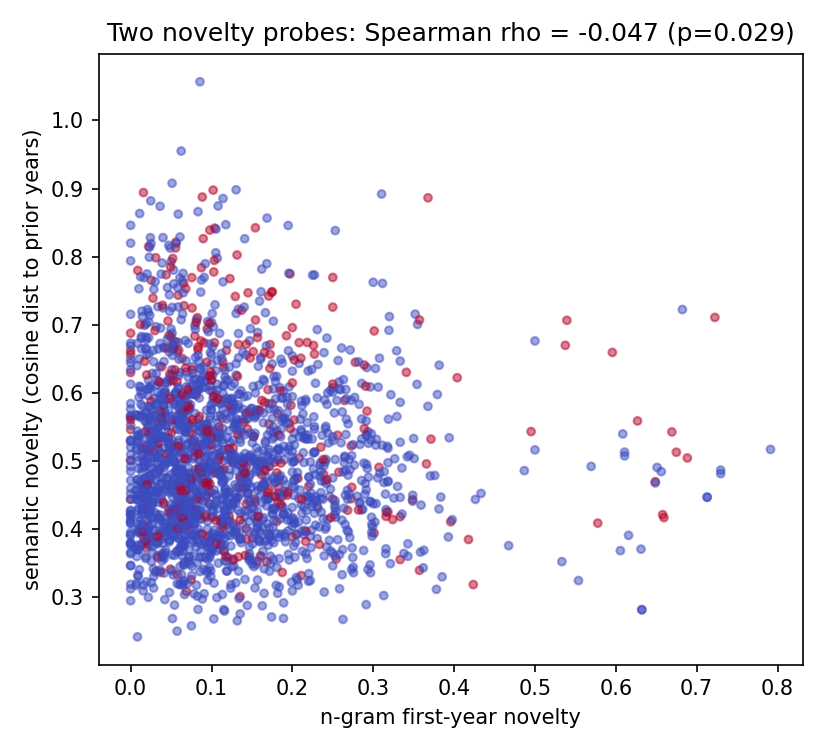
\includegraphics[width=0.55\linewidth]{figures/probe_agreement.png}
\caption{The two novelty probes are nearly orthogonal. Lexical and semantic novelty are not interchangeable.}
\label{fig:probes}
\end{figure}

\subsection{Temporal drift}
We retrained the TF-IDF model with cutoffs $Y \in \{2014, \ldots, 2020\}$ and tested on years $Y+1, Y+2, Y+3$. Mean PR-AUC drops from $0.32$ (gap=1) to $0.31$ (gap=2) to $0.29$ (gap=3); the spread across cutoffs is comparable to the trend, but the direction is consistent. \textbf{The vocabulary of ``what gets cited'' is itself drifting}, which both motivates the temporal split and limits how strong any non-temporal claim could be.

\begin{figure}[h]\centering
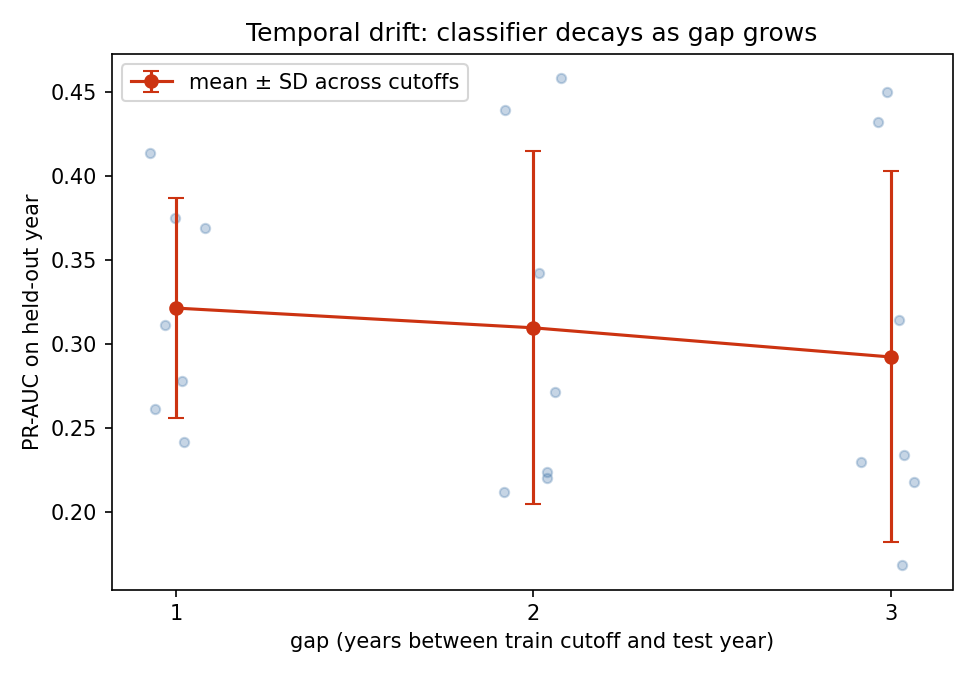
\includegraphics[width=0.6\linewidth]{figures/temporal_drift.png}
\caption{Temporal-drift experiment: PR-AUC of a TF-IDF classifier trained on years $\le Y$, evaluated on year $Y+k$. Each blue dot is one (cutoff, gap) pair; the red curve is the mean over cutoffs at each gap.}
\label{fig:drift}
\end{figure}

\subsection{What the TF-IDF model learned}
\begin{figure}[h]\centering
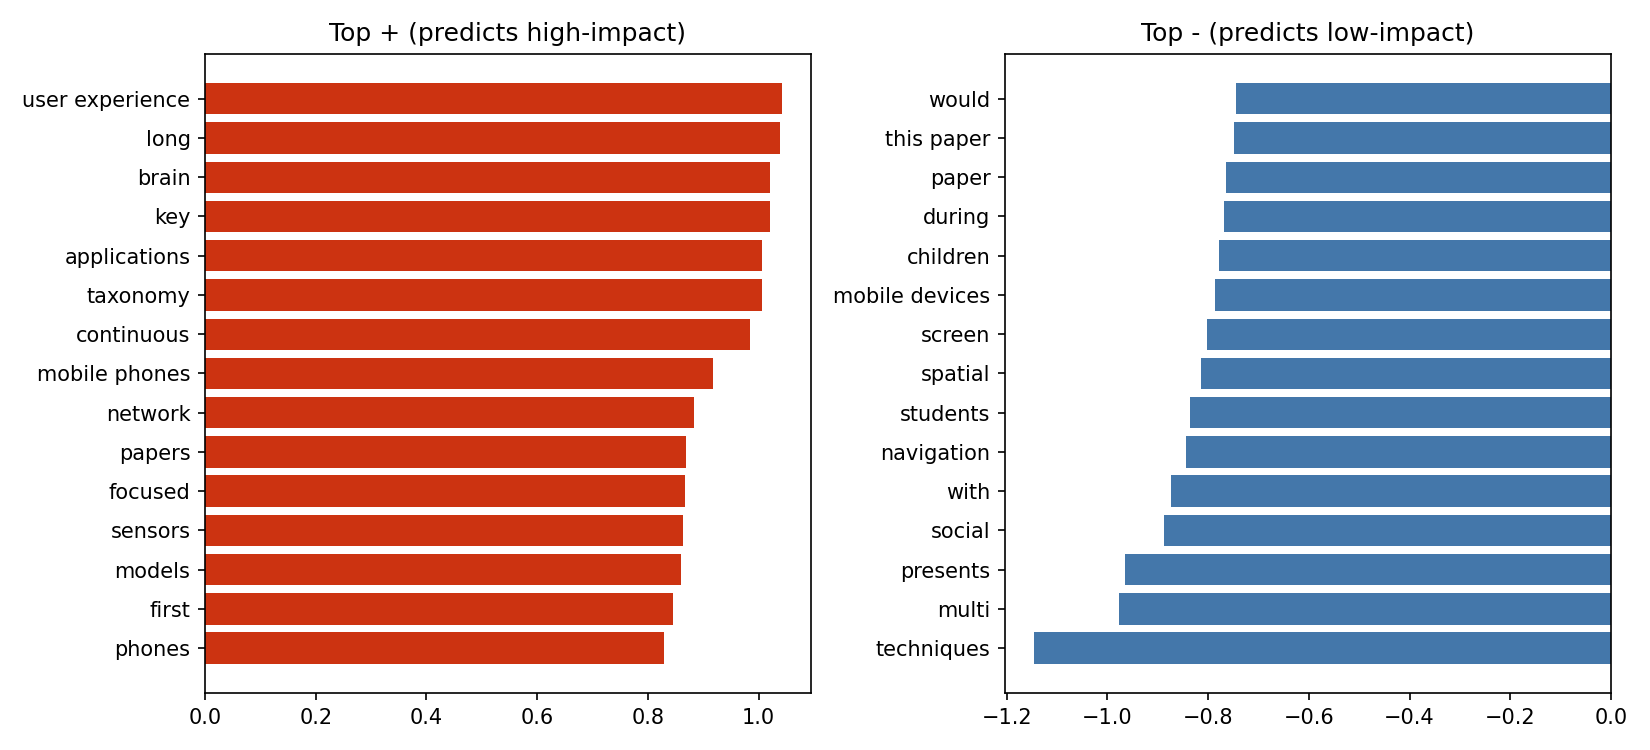
\includegraphics[width=0.95\linewidth]{figures/top_features.png}
\caption{Top 15 most positive and most negative TF-IDF coefficients in the impact classifier. Positive: subfield vocabulary (\texttt{user experience}, \texttt{brain}, \texttt{taxonomy}, \texttt{mobile phones}, \texttt{sensors}). Negative: surface phrases (\texttt{this paper}, \texttt{presents}, \texttt{study}) and crowded sub-areas (\texttt{children}, \texttt{students}, \texttt{navigation}).}
\label{fig:topfeat}
\end{figure}

The pattern is exactly what the probe was designed to expose: the model is rewarding popular topical vocabulary and penalising the writing style of run-of-the-mill papers, not measuring conceptual novelty.

\subsection{Vocabulary growth}
For context, the HCI corpus's cumulative unique-vocabulary curve (Figure~\ref{fig:vocab}) is roughly linear over 2010--2023, indicating that new lexical material is being introduced steadily; this validates that the n-gram novelty probe has signal to detect.

\begin{figure}[h]\centering
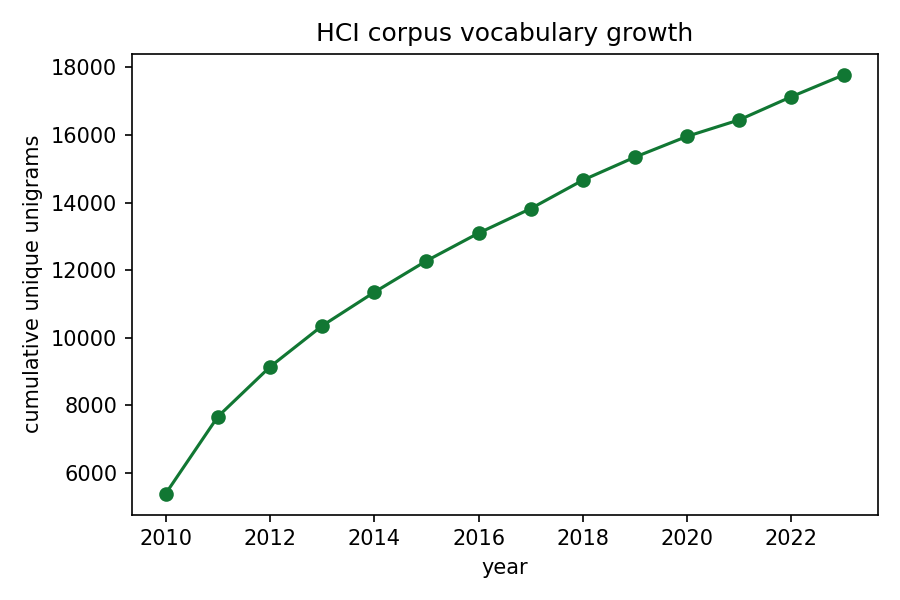
\includegraphics[width=0.55\linewidth]{figures/vocab_growth.png}
\caption{Cumulative unique unigrams (length $\ge 4$) seen in the HCI corpus over time.}
\label{fig:vocab}
\end{figure}

\section{Discussion and limitations}
\begin{enumerate}
  \item \textbf{Selection bias from ingest.} OpenAlex was queried for the top 1{,}600 papers per year by citations. ``Negative'' papers are bottom-half of an above-average pool. This compresses the impact signal and lowers the achievable classification ceiling but does not affect the impact-vs-novelty probe.
  \item \textbf{Both novelty probes are proxies}, and the two disagreeing is itself the report's key qualitative finding---there is no single ``novelty'' quantity.
  \item \textbf{Survey exclusion is regex-based} and may miss surveys whose title doesn't begin with ``a survey of \dots''.
  \item \textbf{Forward generalisation is hard.} Temporal-drift experiment confirms a $\sim$10\% PR-AUC decay per two years of gap, which we report explicitly.
  \item \textbf{Calibration is poor.} Both models are over-confident; a downstream user wanting calibrated probabilities should fit Platt scaling on the validation set.
  \item \textbf{Impact $\ne$ novelty is a finding}, not a weakness. The strongest of our four correlations leaves $>$92\% of variance unexplained.
\end{enumerate}

\section{Conclusion}
Citation-trained text classifiers are not drop-in novelty detectors. On a careful HCI test set, both a strong classical baseline and a modern embedding model produce scores that are at most weakly correlated with two independent corpus-novelty signals, while the two novelty signals themselves are nearly orthogonal. Inspection of feature weights confirms that the classifier learns popular topics and surface style. A 10\% PR-AUC decay per two-year forward gap further argues against treating these models as stable trend detectors. Such classifiers may be useful as a first-pass impact filter, but should not be marketed as novelty detectors and should be paired with term-based and semantic-distance probes when novelty is the intended target.

\section{Reproducibility}
All code is in the project repository under \texttt{src/}. The pipeline (\texttt{pull\_openalex} $\to$ \texttt{filter\_hci} $\to$ \texttt{build\_labels} $\to$ \texttt{model\_tfidf}, \texttt{model\_embed} $\to$ \texttt{novelty\_probe}, \texttt{novelty\_embed} $\to$ \texttt{temporal\_drift} $\to$ \texttt{analysis}, \texttt{analysis\_extended}) is reproducible end-to-end from the provided commands; bootstrap and permutation tests use \texttt{numpy.random.default\_rng(0)}.

\end{document}
